\documentclass{beamer}
\usepackage{ragged2e}
\justifying
\graphicspath{ {./} }
\parindent=1cm
%математика
\usepackage{amssymb,amsmath,mathtext}
\usepackage{indentfirst,amsfonts}
\usepackage{makecell,multirow,longtable}
%язык
\usepackage[english,russian]{babel}
\usepackage[utf8]{inputenc}
% Стиль презентации
\usetheme{Warsaw}
\useoutertheme{infolines}
\begin{document}
\title[Линейные и нелинейные модели]{Линейные и нелинейные модели в задачах автоматической классификации текстов на естественных языках}  
\author[Бочаров И.А.]{Бочаров И.А., А-13-08 \\Научный руководитель: д.т.н., проф. Фальк В.Н.,\\Консультант: Шаграев А.Г.}

\institute[НИУ МЭИ]{НИУ МЭИ, АВТИ, Кафедра Прикладной математики}
\date{Москва, 2014} 
% Создание заглавной страницы
\begin{frame}[plain]
	\titlepage
\end{frame}
% Автоматическая генерация содержания
\begin{frame}
	\tableofcontents
\end{frame}

\section{Цели и задачи}
\begin{frame}
	\tableofcontents[currentsection]
\end{frame}

\begin{frame}
\frametitle{Цель работы}
\textbf{Цель работы:} повышение качества автоматической классификации текстов на естественных языках с применением методов машинного обучения.\\
\end{frame}

\begin{frame}
\frametitle{Решаемые задачи}

\textbf{Решаемые задачи:}
\begin{enumerate}
	\item{Анализ методов предварительной обработки текстовой информации и разработка способа признакового описания документа.}
	\item{Анализ существующих методов решения задачи классификации и модификаций методов решения задачи классификации.}
	\item{Разработка модифицированных версий классических алгоритмов машинного обучения.}
	\item{Сравнительный анализ разработанных автором и известных методов машинного обучения применимо к задаче классификации.}
	\item{Анализ методов сокращения размерности признакового пространства.}
	\item{Разработка метода понижения размерности в задаче классификации текстов.}
\end{enumerate}
\end{frame}

\section{Постановка задачи классификации}
\begin{frame}
	\tableofcontents[currentsection, currentsubsection]
\end{frame}

\begin{frame}
\frametitle{Постановка задачи классификации}
Пусть $X$ - множество классифицируемых объектов, а $Y$ - конечное множество классов. Имеется целевая функция - отображение $y^*:X\rightarrow Y$, значения которой известны только на конечном подмножестве объектов $X' \subset X$ обучающей выборки \\
$$X^l=\{\langle x_i,y_i \rangle |x_i \in X', y_i=y^*(x_i),1\le i \le l\}.$$
\\Необходимо построить решающую функцию $a: X \rightarrow Y$ , принадлежащую
некоторому классу функций $\theta$, которая была бы как можно более качественным
приближением к целевой функции. 
\\Методом обучения $\mu$ будем называть функцию, ставящую в соответствие любой обучающей выборке некоторую
решающую функцию из класса $\theta: \mu(X^l)=a \in \theta.$
\end{frame}

\section{}
\begin{frame}
\frametitle{Признаковое описание документа}
Считаем, что задано непустое множество термов $$W=\{w_1,w_2,...,w_M\},$$
где под термом понимается некоторое слово на естественном языке (возможно, прошедшее некоторый лингвистический анализ). \\
В данной работе используется векторная модель документа:$$d_j=\langle x_j^1,x_j^2,...,x_j^M\rangle,$$ где $x_j^i$ - это вес вхождения $i$-го терма из словаря $W$.\\
Весом вхождения слова $w_i$ в документ $d_j$ называется значение некоторой функции:
$$x_j=f(d_j,w_i)$$
\end{frame}

\section{}
\begin{frame}
\frametitle{Признаковое описание документа}
В данной работе предлагается модифицированная схема выбора весов для слова, явно учитывающая положение вхождений слова в документ. Пусть $d[i]$ - это слово, находящееся в документе $d$ на позиции $i$. Тогда вес слова вычисляется по формуле:
$$f(w_j,d)=\sum\limits_{d[i]=w_j}\gamma(i),$$
где функция $\gamma:\mathbb{N}\rightarrow\mathbb{R}_+$-это некоторая функция одного аргумента.\\
Примеры:
\begin{itemize}
	\item{$\gamma(i)=const;$}
	\item{$\gamma(i)=-\frac{1}{x_{max}}i+b$;}
	\item{...}
\end{itemize}
\end{frame}


\section{Методы классификации}
\subsection{Логистическая регрессия}
\begin{frame}
	\tableofcontents[currentsection, currentsubsection]
\end{frame}

\begin{frame}
\frametitle{Логистическая регрессия}
При использовании метода логистичекой регрессии строится линейная решающая функция вида:
$$a(x,\omega)=sign\left(\sum\limits_{i=1}^M\omega_j x_j-\omega_0\right)=sign\left(\langle x,\omega \rangle\right),$$ где $\langle x,\omega \rangle$ - скалярное произведение векторов $x$ и $\omega$.
\newline
\\Задача обучения логистической регрессии сводится к настройке вектора весов $\omega\in \mathbb{R}^M$ по выборке $X^l$.
\end{frame}

\begin{frame}
\frametitle{Обучение логистической регрессии}
Задача обучения логистической регрессии решается при помощи метода минимизации эмпирического риска с функцией потерь следующего вида:
$$Q(\omega, X^l)=\sum\limits_{i=1}^l ln(1+exp(-y_i\langle x_i,\omega \rangle))\rightarrow \min\limits_{\omega}.$$
\\Вычислим частные производные функции потерь:
$$\frac{\partial Q}{\partial \omega_j}=\sum\limits_{y^*(x_i)=+1}\frac{x_{ij}}{1+exp(\langle x_i,\omega\rangle)}+\sum\limits_{y^*(x_i)=-1}\frac{-x_{ij}}{1+exp(\langle x_i,\omega\rangle)}.$$
\\Получение явных выражений для величин $\omega_j$ из условий $\frac{\partial Q}{\partial \omega_j}=0, j=1..M$ к сожалению, невозможно. Для получения приближенного решения задачи используется метод стохастического градиентного спуска.
\end{frame}

\begin{frame}
\frametitle{Модификации метода логистической регрессии}
\begin{itemize}
	\item{Стратификация\newline 
		На каждом шаге метода стохастического градиентного спуска используются два объекта – один,
		принадлежащий положительному классу, а второй – отрицательному.
	}
	\item{Модификация функционала потерь}
\end{itemize}
\end{frame}

\begin{frame}
\frametitle{Модификация функционала потерь метода логистической регрессии}
	Предлагается ввести смещения в функционал потерь:
	$$Q(\omega, X^l)=\sum\limits_{i=1}^l ln(1+exp(-y_i\langle x_i,\omega \rangle +c))\rightarrow \min\limits_{\omega}.$$
	\\Изменятся значения частных производных:
	$$\frac{\partial Q}{\partial \omega_j}=\sum\limits_{y^*(x_i)=+1}\frac{x_{ij}}{1+exp(\langle x_i,\omega\rangle +c)}+\sum\limits_{y^*(x_i)=-1}\frac{-x_{ij}}{1+exp(\langle x_i,\omega\rangle +c)}.$$
	\\Параметр $c$ становится параметром метода и может быть выбран, к примеру, на основе скользящего контроля.
\end{frame}

\begin{frame}
\frametitle{Положительный эффект от введения смещений}
Приведем на графиках значения величины $\langle x,\omega \rangle$, вычисленные после обучения метода логистической регрессии.
 \begin{columns}[T]
    \begin{column}{.5\textwidth}
    \begin{block}{Без использования смещений}
% Your image included here
    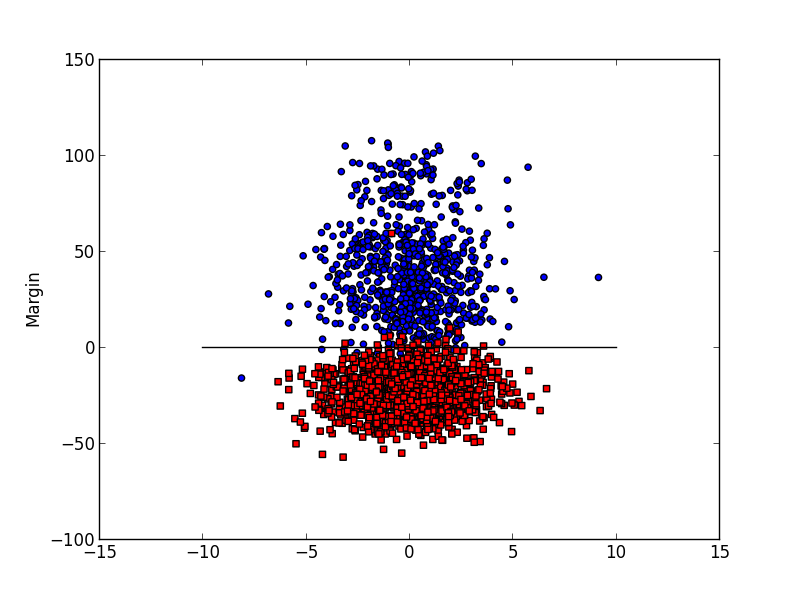
\includegraphics[width=\linewidth,height=\textheight,keepaspectratio]{1.png}
    \end{block}
    \end{column}
    \begin{column}{.5\textwidth}
    \begin{block}{С использованием смещений}
% Your image included here
    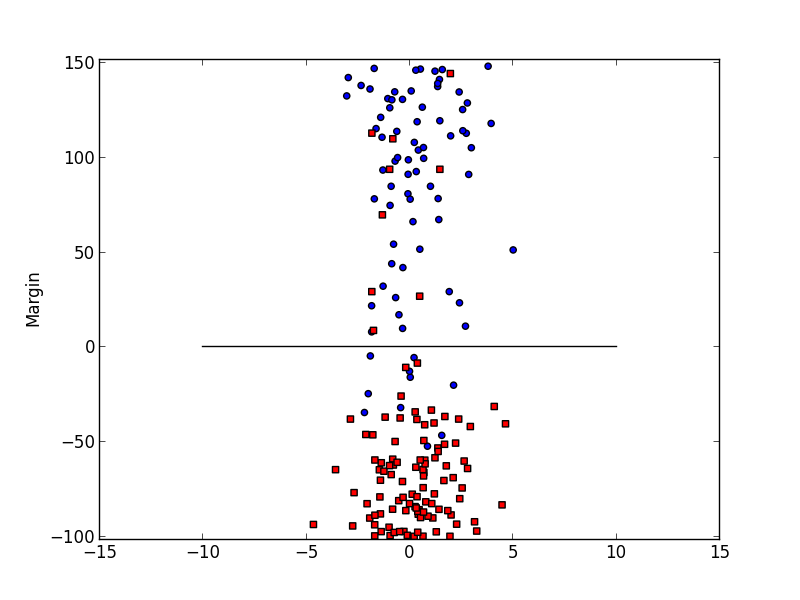
\includegraphics[width=\linewidth,height=\textheight,keepaspectratio]{2.png}
    \end{block}
    \end{column}
  \end{columns}
Приведенные результаты позволяют судить, что использование смещений приводит к более уверенной классификации.
\end{frame}


\subsection{k ближайших соседей}
\begin{frame}
	\tableofcontents[currentsection, currentsubsection]
\end{frame}

\begin{frame}
\frametitle{Построение метода}
Пусть на множестве $X$ введена коммутативная функция расстояния $\rho:X\times X\rightarrow[0,+\infty)$. В этом случае возможно построение разнообразных метрических методов.\\
Для произвольного $u\in X^l$ расположим элементы обучающей выборки в порядке возрастания расстояний до $u$:
$$\rho(u,x_u^{(1)})\le\rho(u,x_u^{(2)})\le ... \le \rho(u, x_u^{(l)}).$$
Пусть $y_u^{(i)}=a(x_u^{(i)})$. Во введенных обозначениях решающее правило метода $k$ ближайших соседей принимает вид $$a(u; X^l, k)=\arg\max\limits_{y \in Y}\sum\limits_{i=1}^{k}[y_u^{(i)}=y],$$
где:
\begin{equation*}
	[X]=
	\begin{cases}
	&1, если\ условие\ X\ выполняется,\\
	&0, в\ противном\ случае.
	\end{cases}
\end{equation*}
\end{frame} 

\begin{frame}
\frametitle{Введение весовых коэффициентов}
Максимум в решающем правиле метода $k$ ближайших соседей может достигаться на нескольких классах. Чтобы избежать неоднозачности, вводится строго убывающая последовательность весов $\omega_i$, задающих вклад $i$-го соседа в классификацию:
$$a(u; X^l, k)=\arg\max\limits_{y \in Y}\sum\limits_{i=1}^{k}[y_u^{(i)}=y]\omega_i.$$\\
При использовании в качестве весов геометрической прогрессии $\omega_i=q^i, q\in(0;1)$ неоднозначностей удается гарантированно избежать. Параметр $q$ становится параметром метода и может быть определен при помощи скользящего контроля.
\end{frame} 

\subsection{Машина опорных векторов (SVM)}
\begin{frame}
	\tableofcontents[currentsection, currentsubsection]
\end{frame}

\begin{frame}
	\frametitle{Машина опорных векторов (SVM)}
	SVM - линейный метод классификации. Основан на построении оптимальной разделяющей гиперплоскости.\\
	Решающее правило метода опорных векторов: $$a(x,\omega)=sign\left(\sum\limits_{i=1}^M\omega_j x_j-\omega_0\right)=sign\left(\langle x,\omega \rangle\right),$$ где $\langle x,\omega \rangle$ - скалярное произведение векторов $x$ и $\omega$.
	\\

	Проблема построения оптимальной разделяющей гиперплоскости сводится к решению задачи квадратичного программирования:
	\begin{equation*}
		\begin{cases}
			&\langle\omega,\omega\rangle\rightarrow\min, \\
			&y_i(\langle\omega,x_i\rangle-\omega_0)\ge1, i=1,...,N
		\end{cases}
	\end{equation*}

	
	$$$$
\end{frame}

\begin{frame}
	\frametitle{Оптимальная разделяющая гиперплоскость}
	\begin{center}
		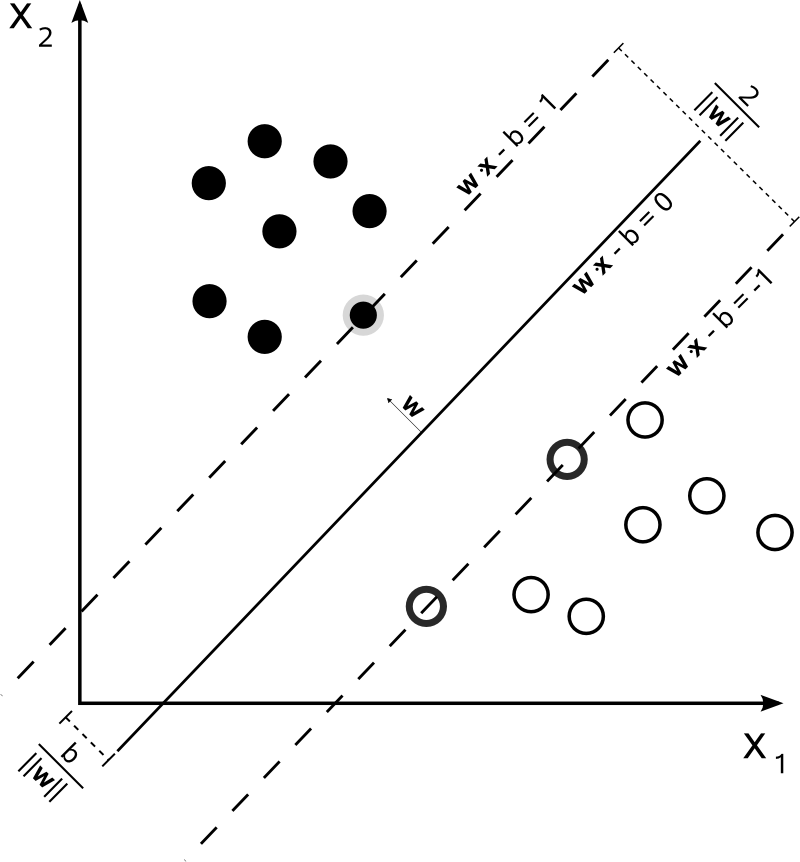
\includegraphics[width=\linewidth,height=.7\textheight,keepaspectratio]{svm_hyperplane.png}
	\end{center}
\end{frame}

\subsection{Деревья решений (Decision Trees, DT)}
\begin{frame}
	\tableofcontents[currentsection, currentsubsection]
\end{frame}

\begin{frame}
\frametitle{Бинарные деревья решений}
Бинарное дерево решений - это алгоритм классификации, задающийся бинарным деревом $\langle E,V\rangle$, в котором каждой внутренней вершине соответствует предикат $\psi'_v:X\rightarrow\{0,1\}$, а каждой терминальной вершине соотвествутет имя класса $y_v\in Y$.
Деревья решений обычно строятся сверху-вниз, на каждом шаге выбирая признак, разбиение по которому наилучшим в некотором смысле образом разделяет выборку.\newline\\
Наиболее употребительные критерии:
\begin{itemize}
	\item{Gini impurity.}
	\item{Критерий информативности.}
\end{itemize}
\end{frame}

\begin{frame}
\frametitle{Критерии разбиения}
Пусть имеется $m$ классов: $Y={y_1,y_2,...,y_m}$, а величина $f_i=\frac{|Y_i|}{|Y|}$ - доля объектов $i$-го класса в некотором множестве прецедентов.\newline
\\Во введенных обозначениях:
\begin{itemize}
	\item{$I_G(f)=1-\sum\limits_{i=1}^{m}{f_i}^2$ - Gini Impurity. Используется в CART-деревьях.}
	\item{$I_E(f)=-\sum\limits_{i=1}^{m}{f_i}\log_2f_i$ - Информативность. Используется в алгоритмах ID3 и C4.5.}
	
\end{itemize}

\end{frame}

\section{Сокращение размерности признакового пространства}
\begin{frame}
	\tableofcontents[currentsection, currentsubsection]
\end{frame}

\begin{frame}
\frametitle{Методы сокращения размерности}
	\begin{itemize}
		\item{Отбор признаков}
			\begin{itemize}
			\item{Полный перебор}
			\item{Последовательное добавление/удаление признаков}
			\item{Кластеризация признаков}
			\item{Генетические алгоритмы}
			\end{itemize}
		\item{Синтез признаков}
			\begin{itemize}
			\item{Метод главных компонент, PCA}
			\item{Нейросетевой подход к синтезу признаков}
			\end{itemize}
	\end{itemize}\leavevmode\newline
	\\Предлагается использовать нейронную сеть в качестве метода сокращения размерности в задаче классификации текстов.
\end{frame}

\begin{frame}
\frametitle{Разреженный автоэнкодер(spatial autoencoder)}
% \begin{columns}[T]
%     \begin{column}{.5\textwidth}
%     \begin{block}{Структура автоэнкодера}
%     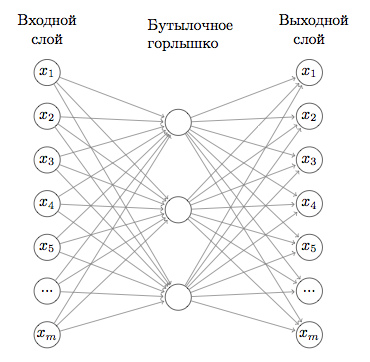
\includegraphics[width=\linewidth,height=.7\textheight,keepaspectratio]{autoencoder.png}
%     \end{block}
%     \end{column}
%  \end{columns}
\begin{center}
	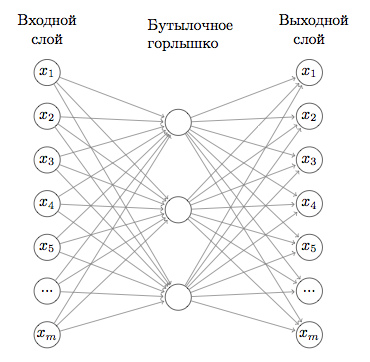
\includegraphics[width=\linewidth,height=.7\textheight,keepaspectratio]{autoencoder.png}
\end{center}
\end{frame}

\begin{frame}
\frametitle{Модификация автоэнкодера}
% \begin{columns}[T]
%     \begin{column}{1\textwidth}
%     \begin{block}{Структура модифицированного автоэнкодера}
%     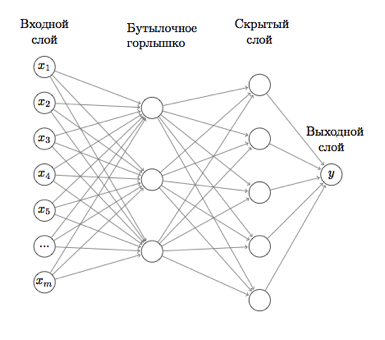
\includegraphics[width=\linewidth,height=.7\textheight,keepaspectratio]{modified_encoder.png}
%     \end{block}
%     \end{column}
%   \end{columns}
\begin{center}
	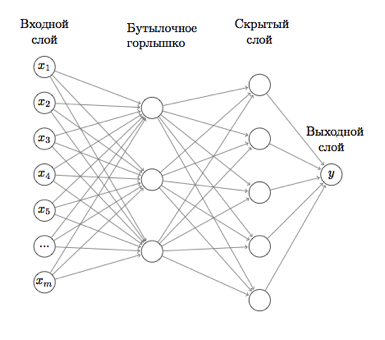
\includegraphics[width=\linewidth,height=.7\textheight,keepaspectratio]{modified_encoder.png}
\end{center}
\end{frame}


\section{Оценка качества классификации}
\begin{frame}
	\tableofcontents[currentsection, currentsubsection]
\end{frame}

\begin{frame}
\frametitle{Оценка качества классификации}
Для измерения качества предсказаний необходимо определить функционал
качества – функцию, которая всякому набору прецедентов (пар, состоящих из
объектов и соответствующих им ответов) и решающей функции сопоставляет
некоторое число. Считается, что, чем больше значение функционала качества, тем лучше качество предсказаний решающей функции.
\newline
\newline
\\
Пусть $X^t$-тестовая выборка. Тогда значение функционала $$Q(X^t,\mu(X^l))$$ можно считать оценкой обобщающей способности метода обучения $\mu$.
\end{frame}


\begin{frame}
\frametitle{Скользящий контроль}
	Пусть имеется обучающая выборка $X^l$, метод обучения $\mu$ и некоторый функционал качества $Q$. Зафиксируем множество разбиений выборки $X^l$:
	$$\{\{S_1^l,S_1^t\},\{S_2^l,S_2^t\},...,\{S_k^l,S_k^t\}\},$$
	$$S_i^l \cup S_i^t = X^l, i=1..k.$$
	Оценка качества, усредненная по всем разбиениям, называется оценкой скользящего контроля:
	$$CV(Q,\mu,S)=\frac{1}{k}\sum\limits_{i=1}^{k}Q(S_i^t,\mu(S_i^l)).$$
\end{frame}

\begin{frame}
\frametitle{Стратификация выборки}
	Желательно, чтобы разбиения, используемые при получении оценок методом скользящего контроля обладали теми же статистическими свойствами, что и вся выборка $X^l$. Для достижения этого часто используется стратификация.
	\newline
	\newline
	Стратификация классов заключается в том, что разбиения проводятся таким образом, что доля каждого класса $k$ в каждой подвыборке $X_i^l$ примерно равна:
	$$\frac{|X_i^l|}{|X^l|}\sum\limits_{\langle x,y \rangle \in X^l}^{}[y=k].$$
\end{frame}

\section{Вычислительные эксперименты}
\begin{frame}
	\tableofcontents[currentsection, currentsubsection]
\end{frame}

\begin{frame}
\frametitle{Эксперимент №1. Влияние предобработки на качество классификации}
\begin{center}
    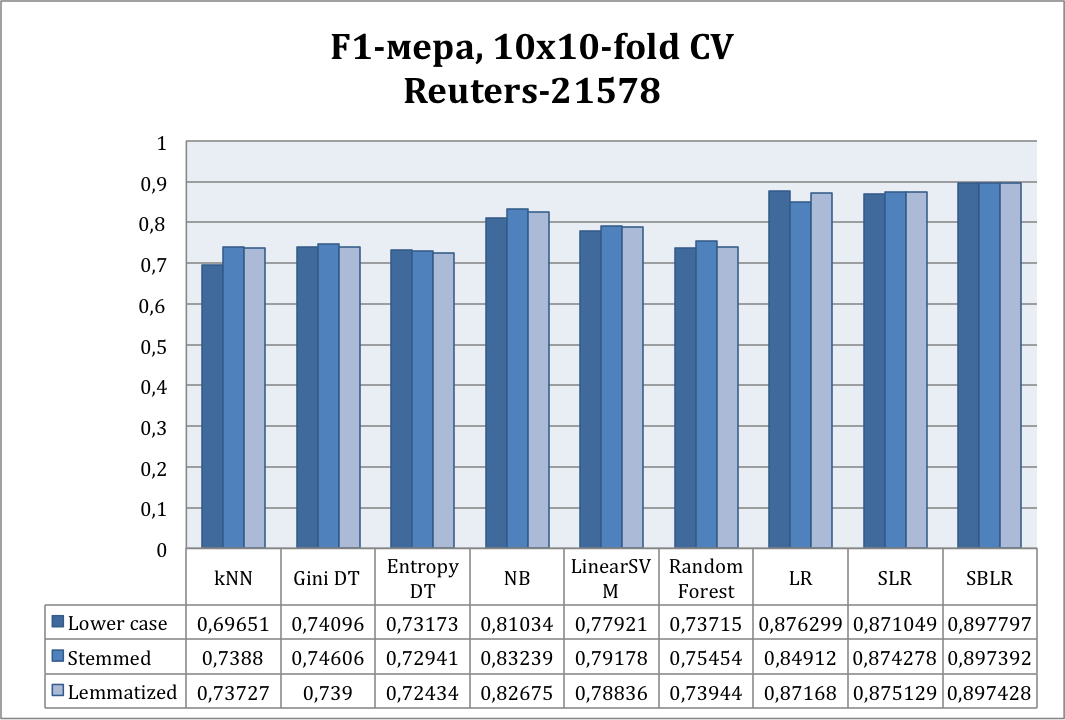
\includegraphics[width=\linewidth,height=0.7\textheight,align=\center,keepaspectratio, trim=4 4 4 4, clip]{reuters-preprocessing.png}
\end{center}
\end{frame}

\begin{frame}
\frametitle{Эксперимент №1. Влияние предобработки на качество классификации}
\begin{columns}[T]
    \begin{column}{.5\textwidth}
    %\begin{block}{Использование стемминрга}
% Your image included here
    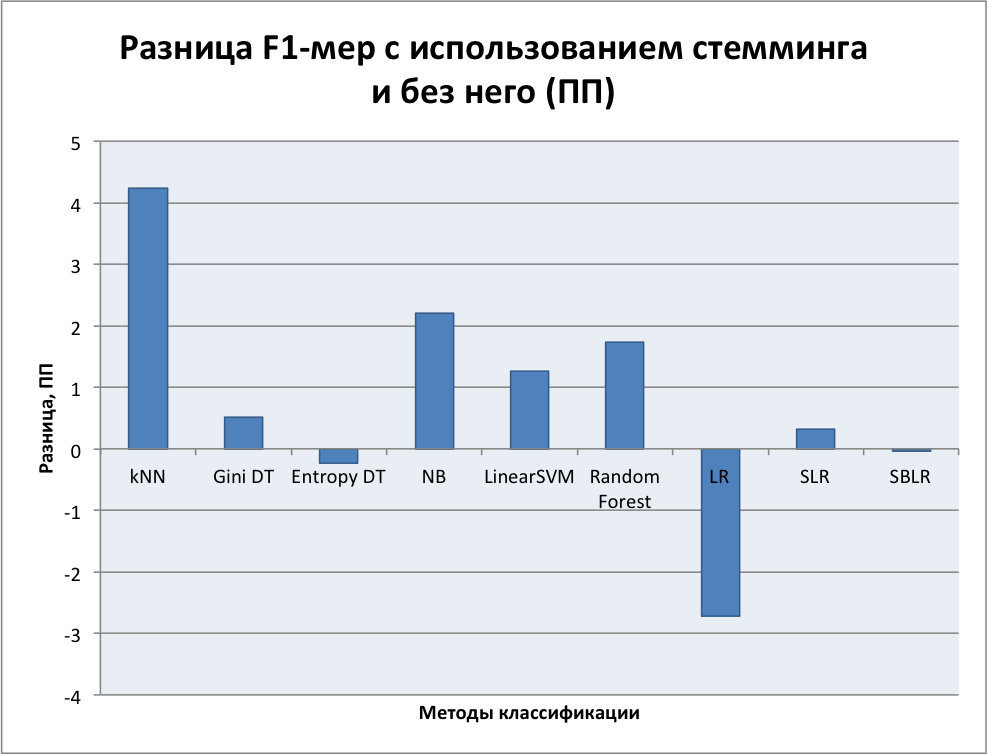
\includegraphics[width=\linewidth,height=\textheight,keepaspectratio, trim=4 4 4 4, clip]{stemming-diff.png}
    %\end{block}
    \end{column}
    \begin{column}{.5\textwidth}
    %\begin{block}{Использование лемматизатора}
% Your image included here
    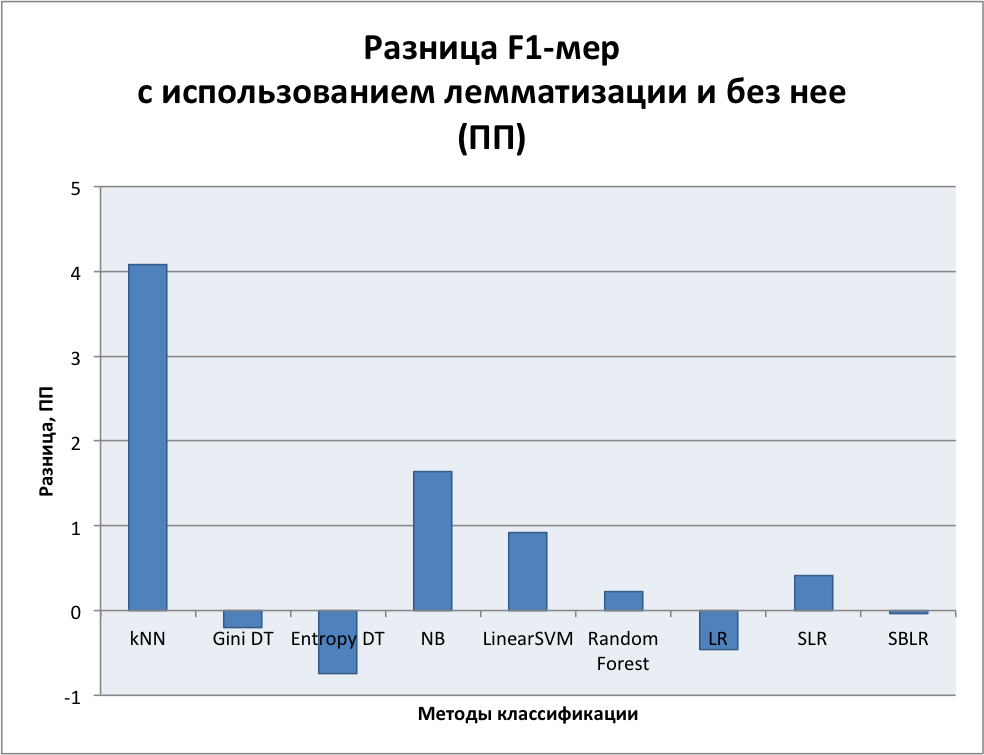
\includegraphics[width=\linewidth,height=\textheight,keepaspectratio, trim=4 4 4 4, clip]{lemmatizing-diff.png}
    %\end{block}
    \end{column}
  \end{columns}
\end{frame}

\begin{frame}
\frametitle{Эксперимент №2. Выбор схемы взвешивания вхождения слов в документы}
Для задачи классификации текстовых докуметнтов, учитывая особенности строения новостных текстов,
выберем следующие функции для использования в схеме вычисления весов:
\newline
\\
\begin{itemize}
	\item{константный вес: $\gamma(i)=const$;}
	\item{линейно убывающий вес: $\gamma(i)=-\frac{1}{x_{max}}i+b$;}
	\item{гиперболический вес: $\gamma(i)=\frac{k_1}{i}$;}
	\item{вес-"сигмоида": $\gamma(i)=\frac{1+e^{-k_1*k_2}}{1+e^{-k_1*(k_2+1-i)}}$.}
\end{itemize}
\end{frame}

\begin{frame}
\frametitle{Эксперимент №2. Выбор схемы взвешивания вхождения слов в документы}
\begin{center}
    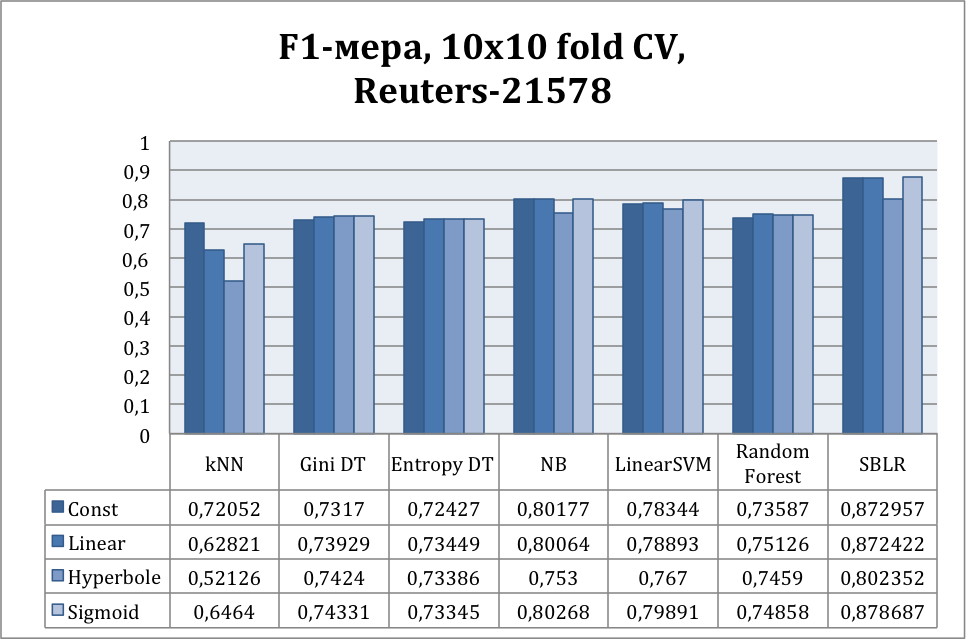
\includegraphics[width=\linewidth,height=0.7\textheight,align=\center, trim=4 4 4 4, clip, keepaspectratio]{weighting.png}
\end{center}
\end{frame}

\begin{frame}
\frametitle{Эксперимент №2. Выбор схемы взвешивания вхождения слов в документы}
\begin{center}
    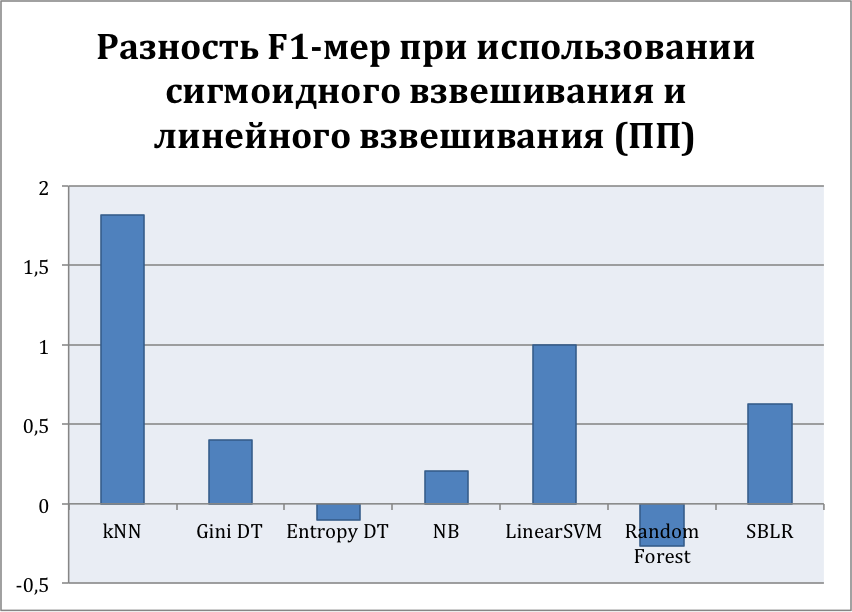
\includegraphics[width=\linewidth,height=0.7\textheight,align=\center,trim=4 4 4 4, clip, keepaspectratio]{lin-sigm-diff.png}
\end{center}
\end{frame}

\begin{frame}
\frametitle{Эксперимент №3. Использование нейронной сети в качестве метода для синтеза признаков}
\begin{center}
    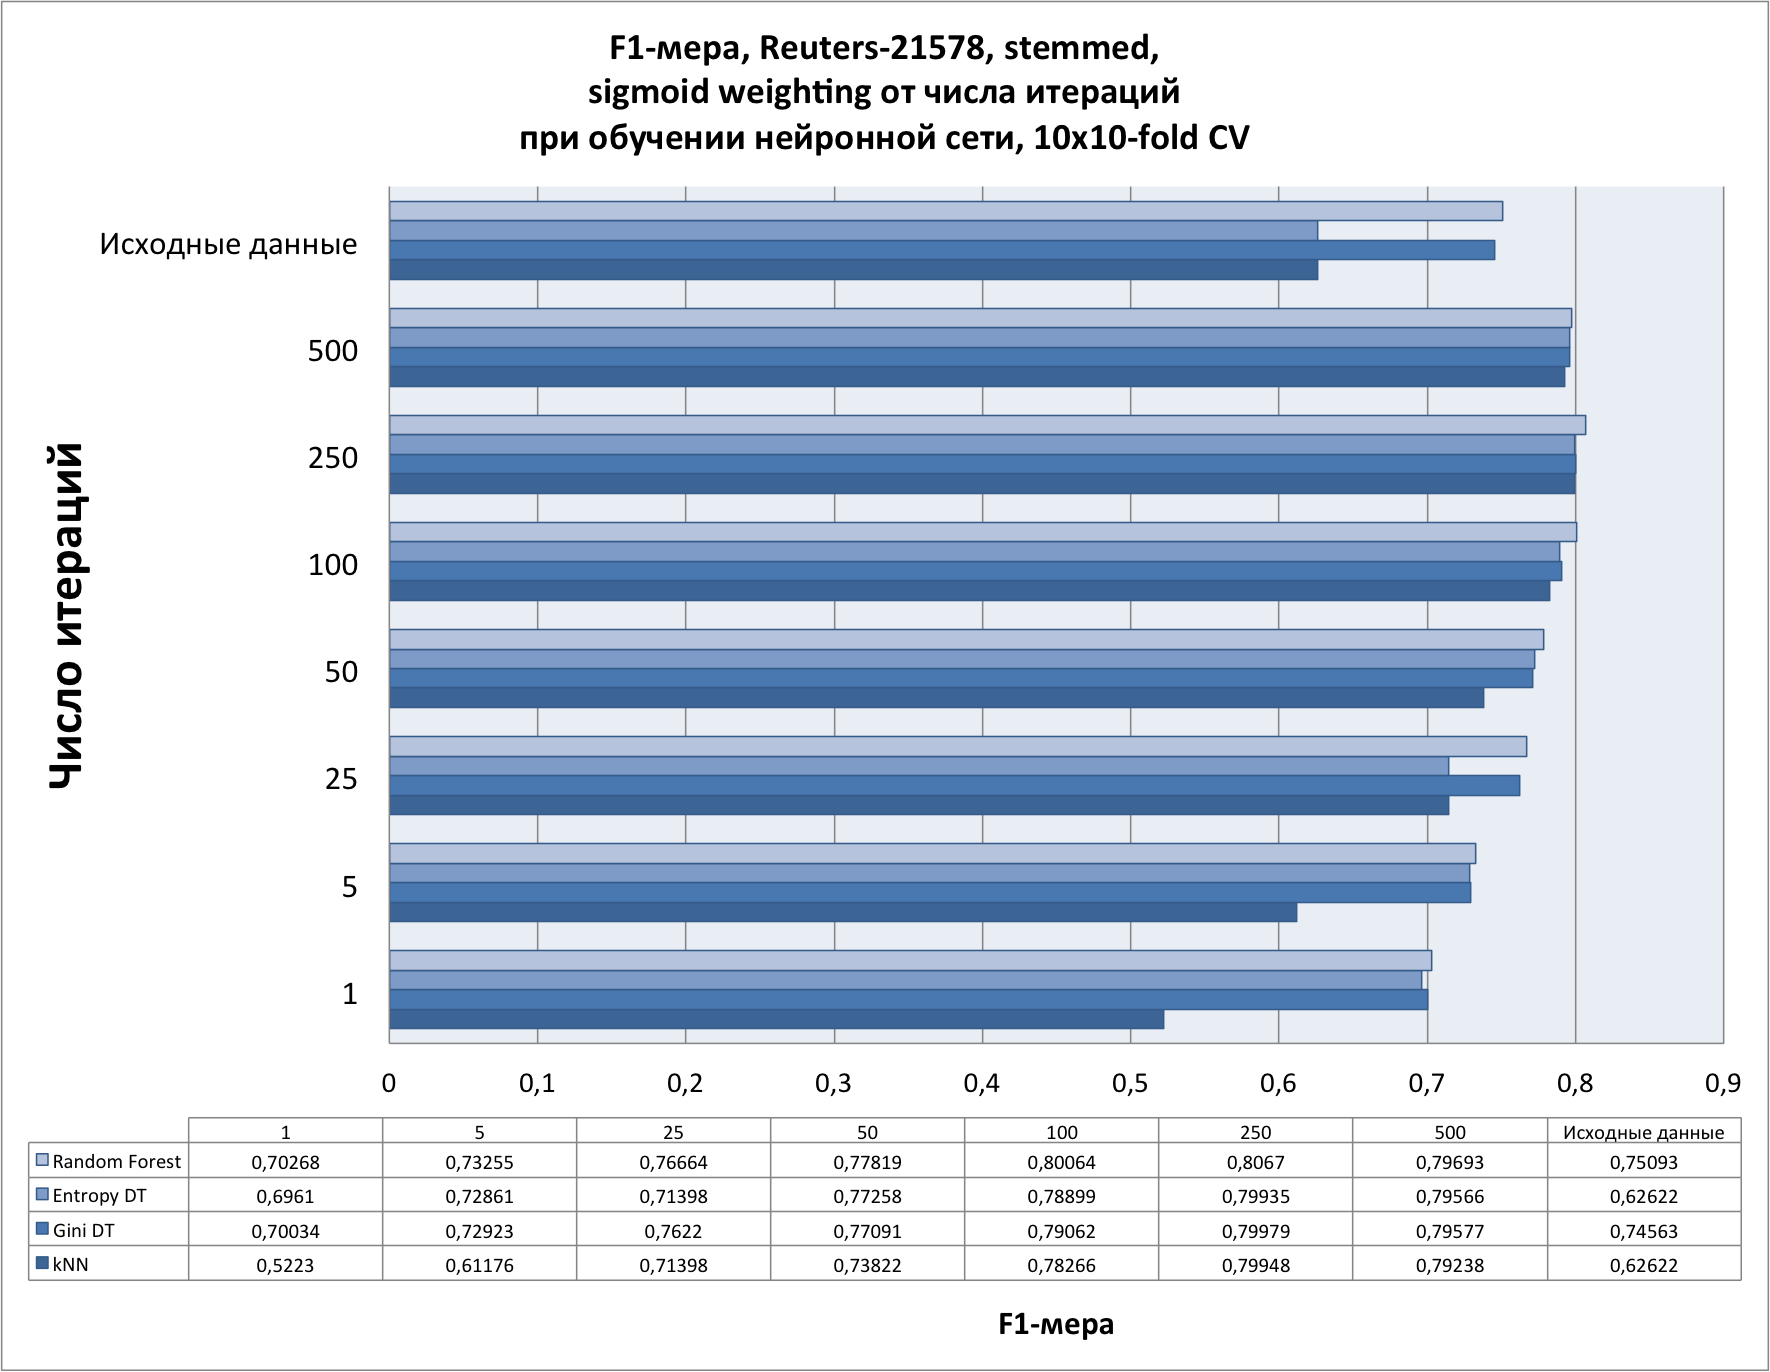
\includegraphics[width=\linewidth,height=0.8\textheight,align=\center,trim=4 4 4 4, clip, keepaspectratio]{neural-reuters.png}
\end{center}
\end{frame}

\begin{frame}
\frametitle{Эксперимент №4. Сравнение типов автоэнкодеров}
\begin{center}
    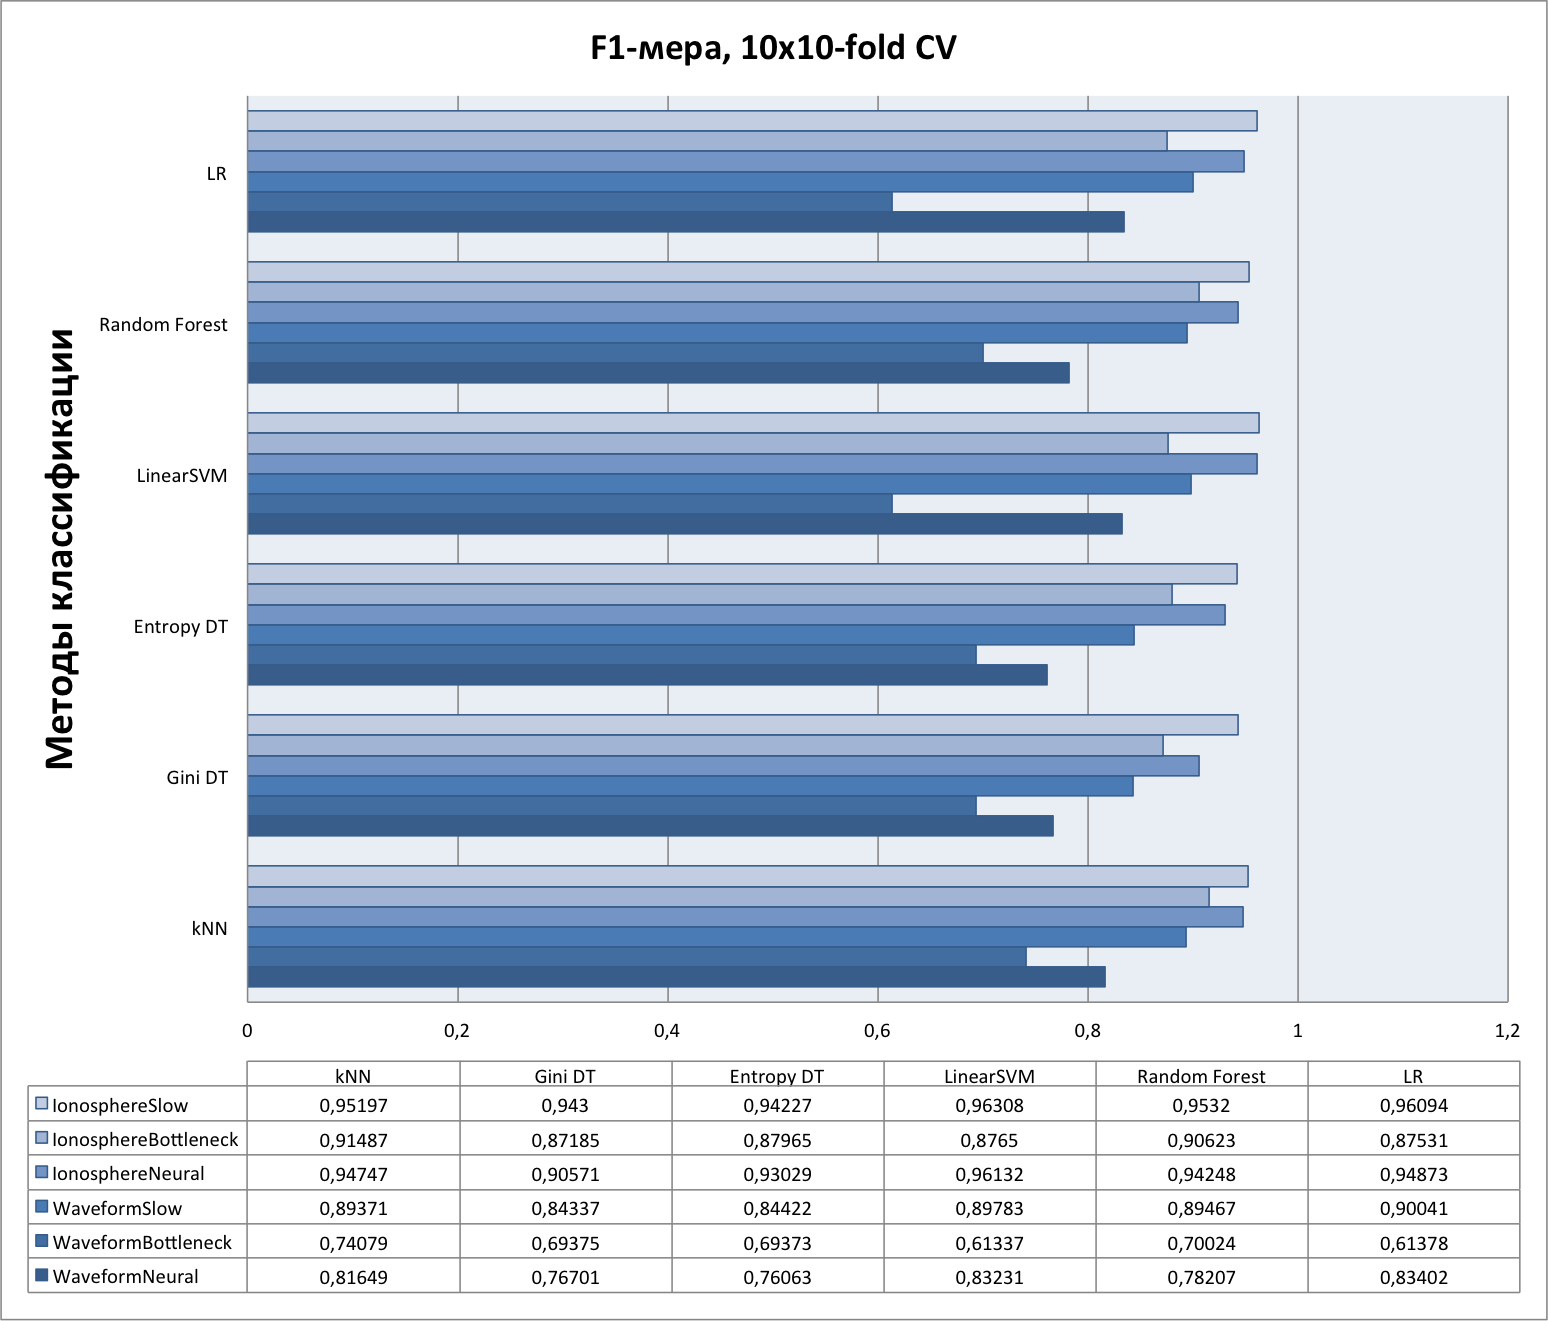
\includegraphics[width=\linewidth,height=0.8\textheight,align=\center,trim=4 4 4 4, clip, keepaspectratio]{autoencoder-comparison.png}
\end{center}
\end{frame}

\begin{frame}
\frametitle{Результаты применения разных методов классификации. Reuters-21578}
\begin{center}
    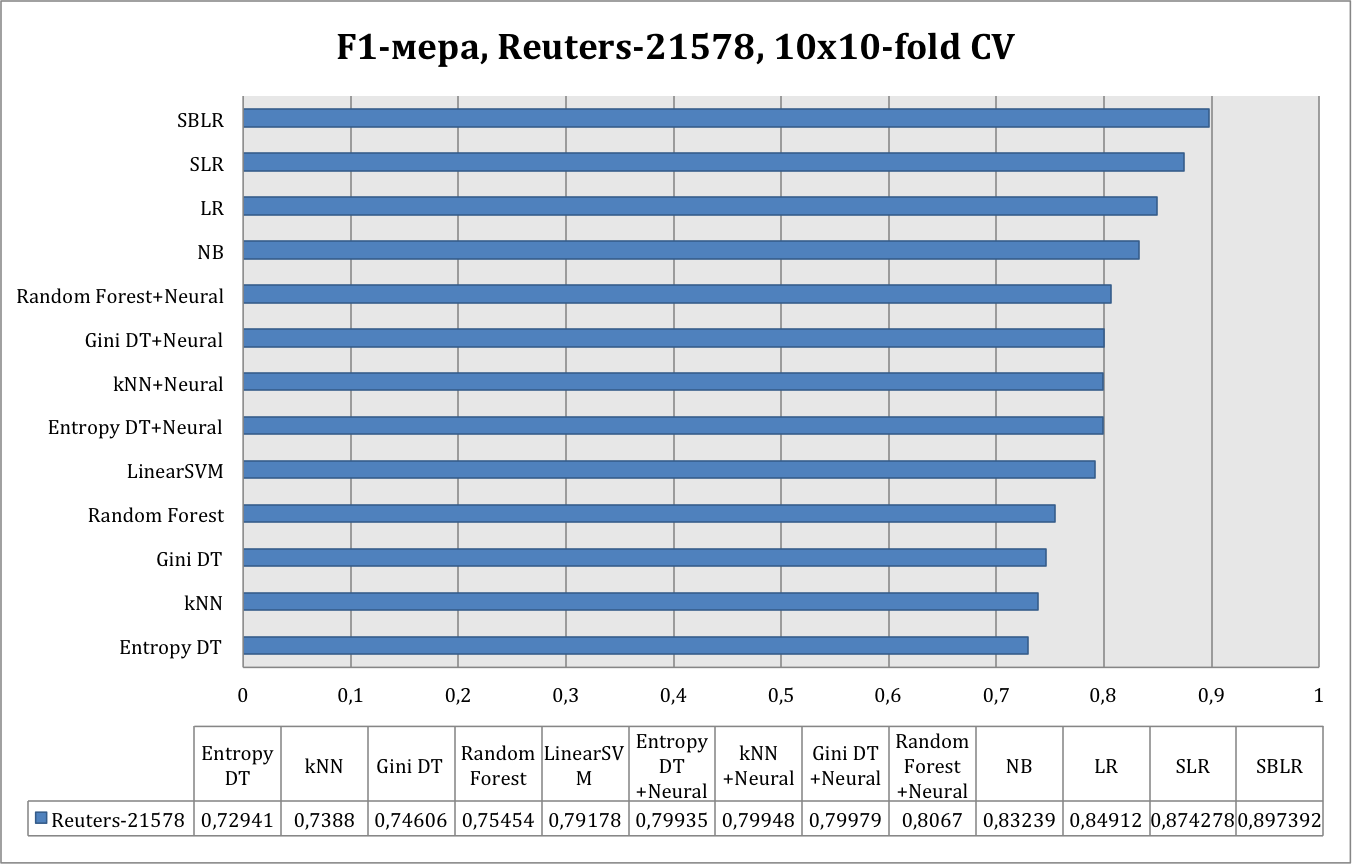
\includegraphics[width=\linewidth,height=0.75\textheight,align=\center,trim=4 4 4 4, clip, keepaspectratio]{reuters-summary.png}
\end{center}
\end{frame}

\section{Результаты}
\begin{frame}
	\tableofcontents[currentsection, currentsubsection]
\end{frame}

\begin{frame}
\frametitle{Результаты}
\begin{itemize}
	\item{Проведен анализ методов предварительной обработки текстовой информации.}
	\item{Разработан способ формирования признакового описания документа.}
	\item{Проанализированы существующие методы решения задачи классификации, рассмотрены модификации классических методов.}
	\item{Реализованы модифицированные версии классических алгоритмов.}
	\item{Предложен эффективный способ сокращения размерности признакового пространства с использованием нейронных сетей.}
	\item{Проведен ряд вычислительных экспериментов, позволяющих судить о практической ценности рассмотренных методов классификации.}
\end{itemize}
\end{frame}



\section{}
\begin{frame}
\frametitle{Спасибо за внимание!}
	\begin{center}
		Спасибо за внимание!
	\end{center}
\end{frame}

\end{document}
